The study of soft observables in high-multiplicity p-Pb (and even p-p) collisions led to the observation of signals qualitatively, and often also quantitatively, very similar to the ones measured in nucleus-nucleus collisions and traditionally attributed to the formation of a hot deconfined medium displaying a collective behaviour: long-range azimuthal 2-particle correlations~\cite{Khachatryan:2010gv,CMS:2012qk,Abelev:2012ola,Aad:2012gla}, non-vanishing flow harmonics~\cite{ABELEV:2013wsa,Khachatryan:2015waa}, increasing baryon/meson ratio as a function of $p_T$, enhancement of strange-hadron production...Many authors interpreted these observation as indications that the same strongly-interacting medium, with a collective hydrodynamic expansion driven by pressure gradients, supposed to be formed in nucleus-nucleus collisions is also produced in the case of small systems. If the hydrodynamic scheme provides a consistent framework capable of describing essentially all the above observations, its strong underlying assumptions, i.e. the realization of a system not too far from local thermal equilibrium with a mean-free-path much smaller than its size ($\lambda_{\rm mfp}\ll L$), looks challenging for the case of small systems like the ones produced in proton-nucleus collisions. Hence some authors looked for alternative interpretation of the data -- in particular the ones related to particle correlations and flow harmonics -- in terms, for instance, of initial-state effects (Color-Glass-Condensate~\cite{Dusling:2013qoz}), of the formation of a system with small parton-parton cross-sections~\cite{Bzdak:2014dia} or of quantum-mechanical interference in the presence of multiple sources of particle production, entailing to reconsider the no-interaction baseline before looking for final-state collective effects~\cite{Blok:2017pui}.

On the other hand no signature of jet-quenching or suppression of high-$p_T$ particle production was observed in high-multiplicity proton-nucleus collisions. At first glance this may look in contradiction with the interpretation of the  measurements involving soft observables, in terms of non-trivial final-state medium effects. One should in any case consider that the quenching of jets due to parton energy-loss in the QGP has a strong dependence on thickness of the crossed matter (one has $\Delta E\sim \alpha_s\hat q L^2$ for the average energy-loss due to medium-induced gluon radiation). On the contrary, if one accepts the hydrodynamic paradigm, the smaller size of the medium with respect to the nucleus-nucleus case would lead to even larger initial pressure gradients and hence to a larger collective acceleration of the fluid, able to compensate its shorter lifetime. Hence, although reproducing within a unified theoretical framework the apparently opposite observations in the low-$p_T$ and high-$p_T$ sectors looks challenging, the latter are not necessarily in contradiction.

In light of the above findings it is clearly of interest to address the study of light systems also through heavy-flavour observables. Due to their large mass $c$ and $b$ quarks are in fact produced in the very first instants in hard processes described by pQCD, at most affected by nuclear modifications of the Parton Distribution Functions (nPDF's) and by an initial transverse-momentum broadening acquired in Cold Nuclear Matter. Since the large mass suppresses also the excitation of $Q\bar Q$ pairs from the vacuum during hadronization, any detected heavy-flavour hadron certainly carries $c$ or $b$ quarks produced during the initial collision and which has crossed the possibly produced medium. It looks then natural to extend transport calculations developed to describe heavy-flavour production in nucleus-nucleus collisions to provide theoretical predictions also in the case of small systems, assuming that also in this case a hot deconfined medium is formed. The theoretical modelling involves the same processes as in the heavy-ion case: the so-called Cold-Nuclear-Matter effects (nPDF's and initial $k_T$-broadening) modifying the hard $Q\overline{Q}$ production, the propagation of the heavy quarks throughout the fireball and finally their hadronization in the presence of a hot medium. The only difference is that it becomes now mandatory to include event-by-event fluctuations in the initial conditions, since, at variance with the nucleus-nucleus case, the centrality and eccentricity of the collision is no longer essentially fixed by the impact parameter. 

\begin{figure}[ht]
\centering
%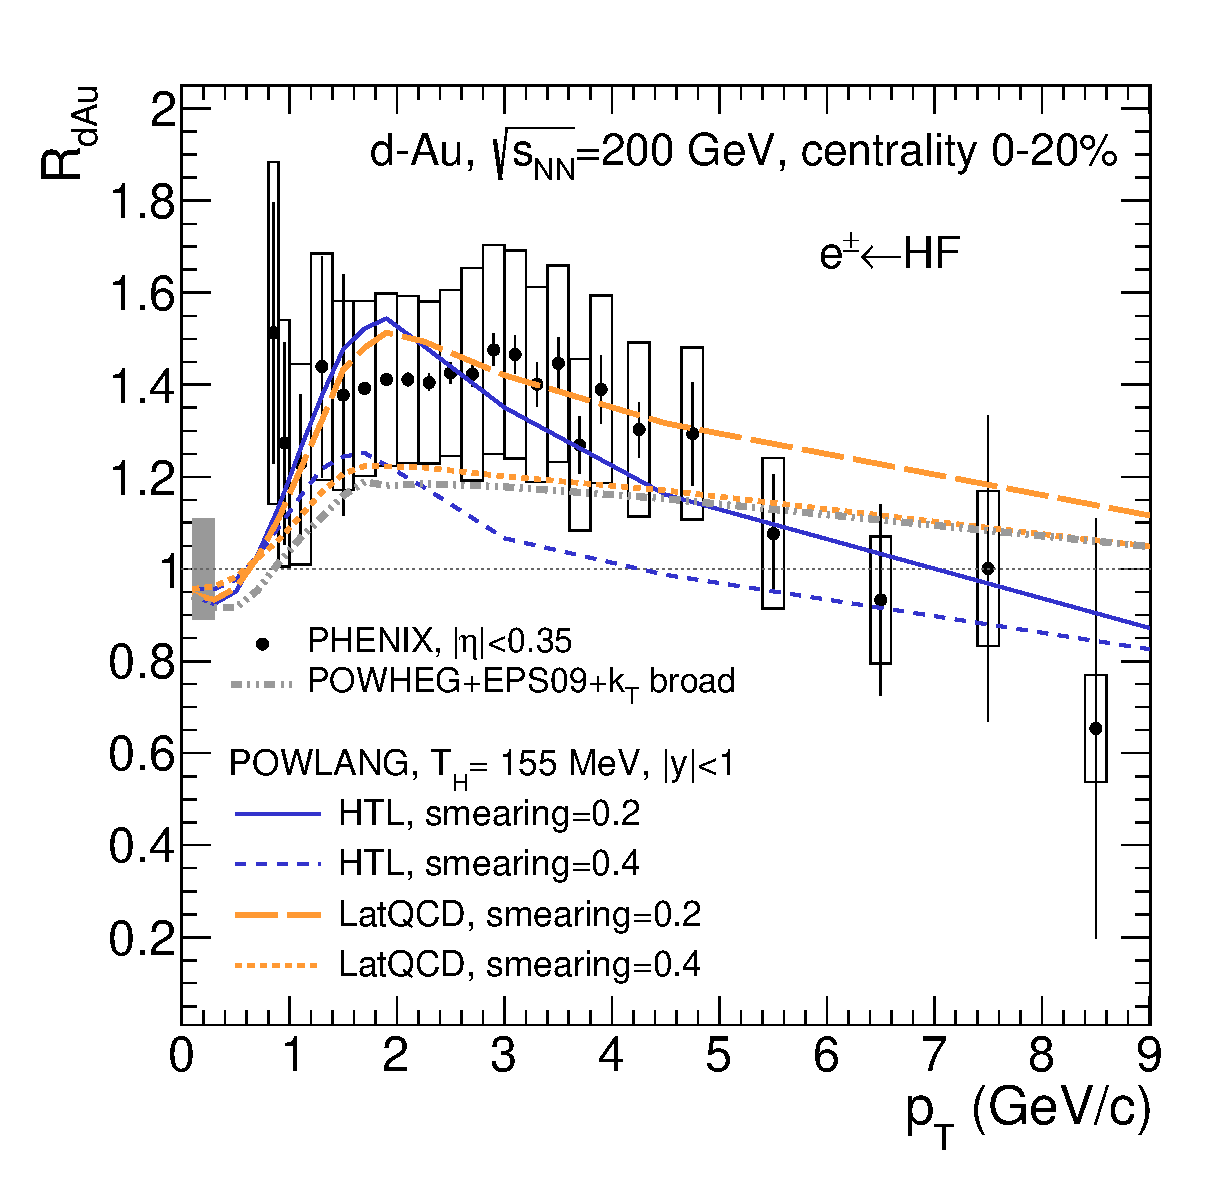
\includegraphics[width=0.49\textwidth]{hf/figures/RHIC_RdAu_HFE_020_HTLvsLATvsNuclPOWHEG_PHENIX.eps}
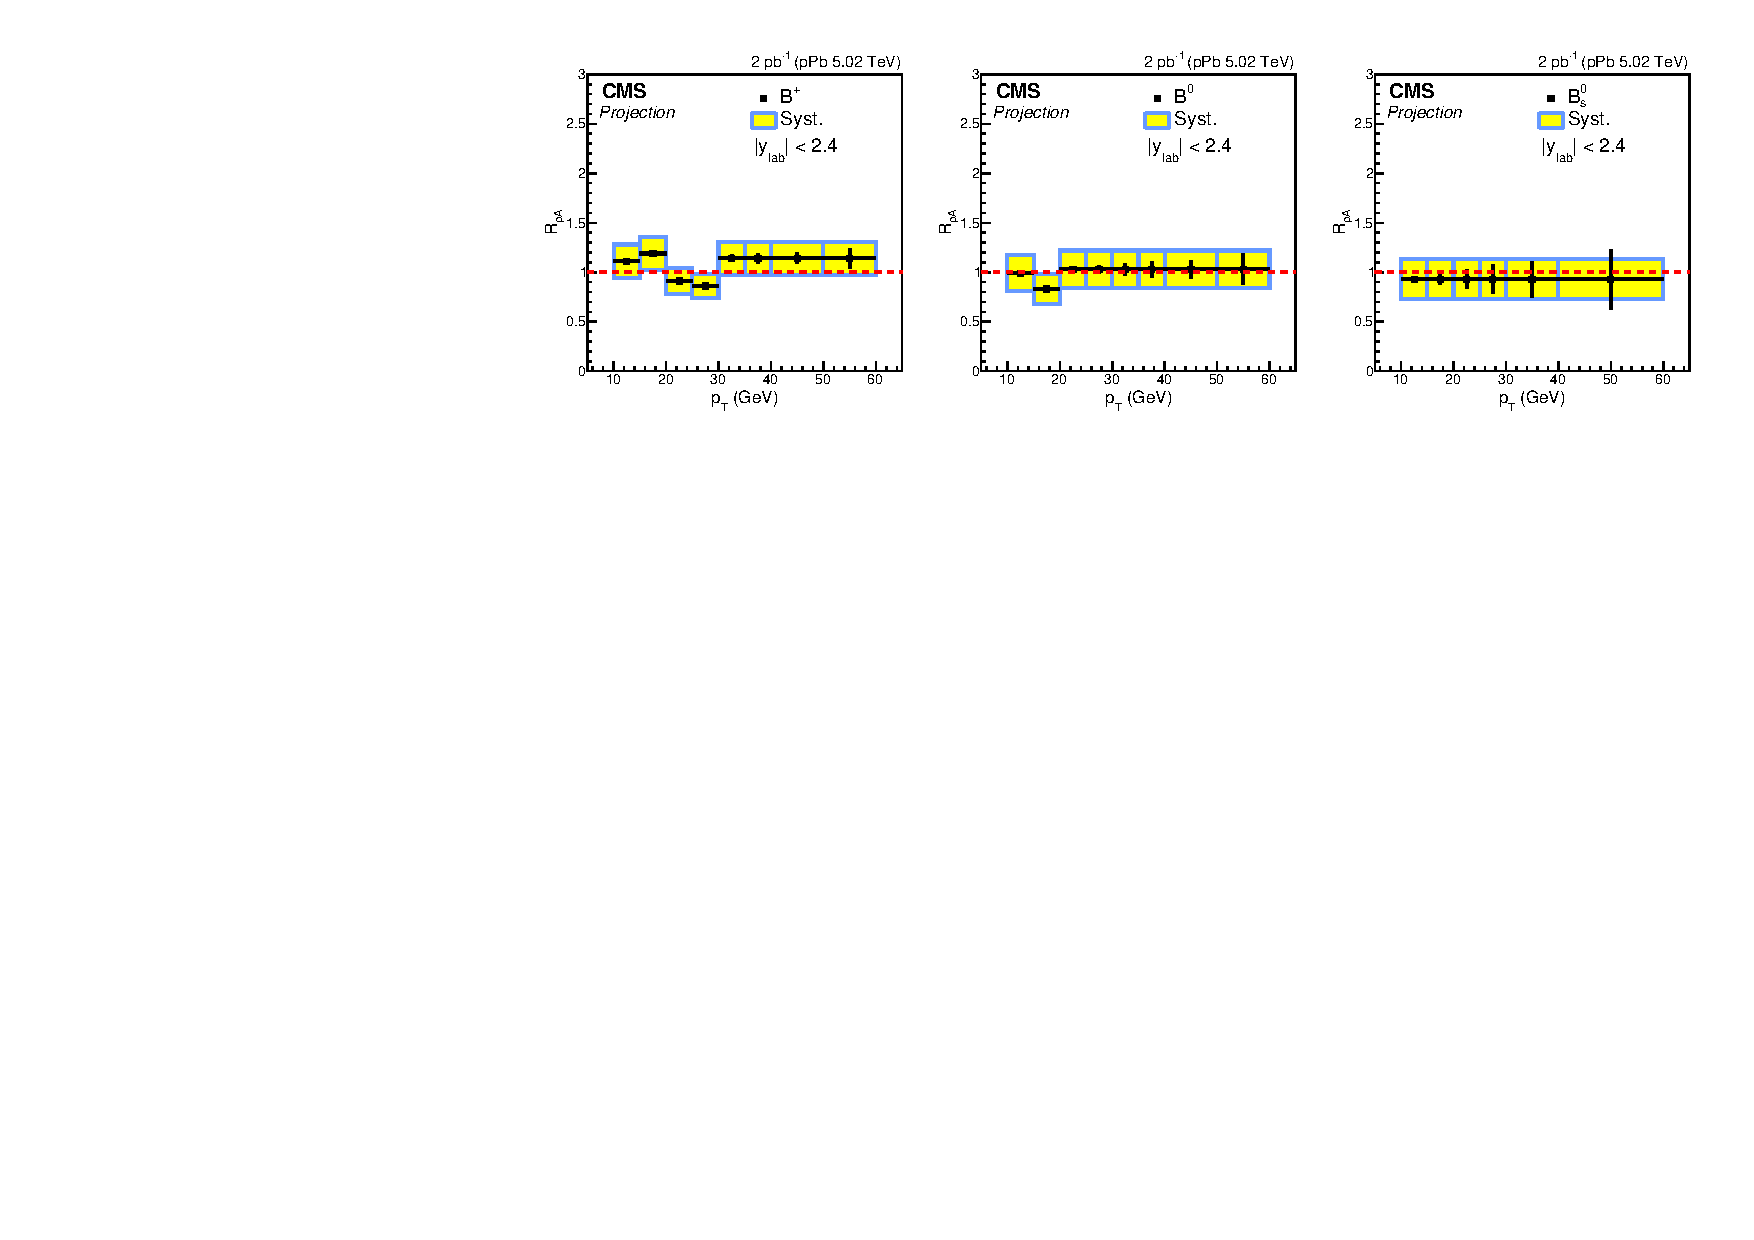
\includegraphics[trim=00 13cm 0,clip,width=0.4\textwidth]{hf/figures/cRpA_lumiTG_2000.pdf}
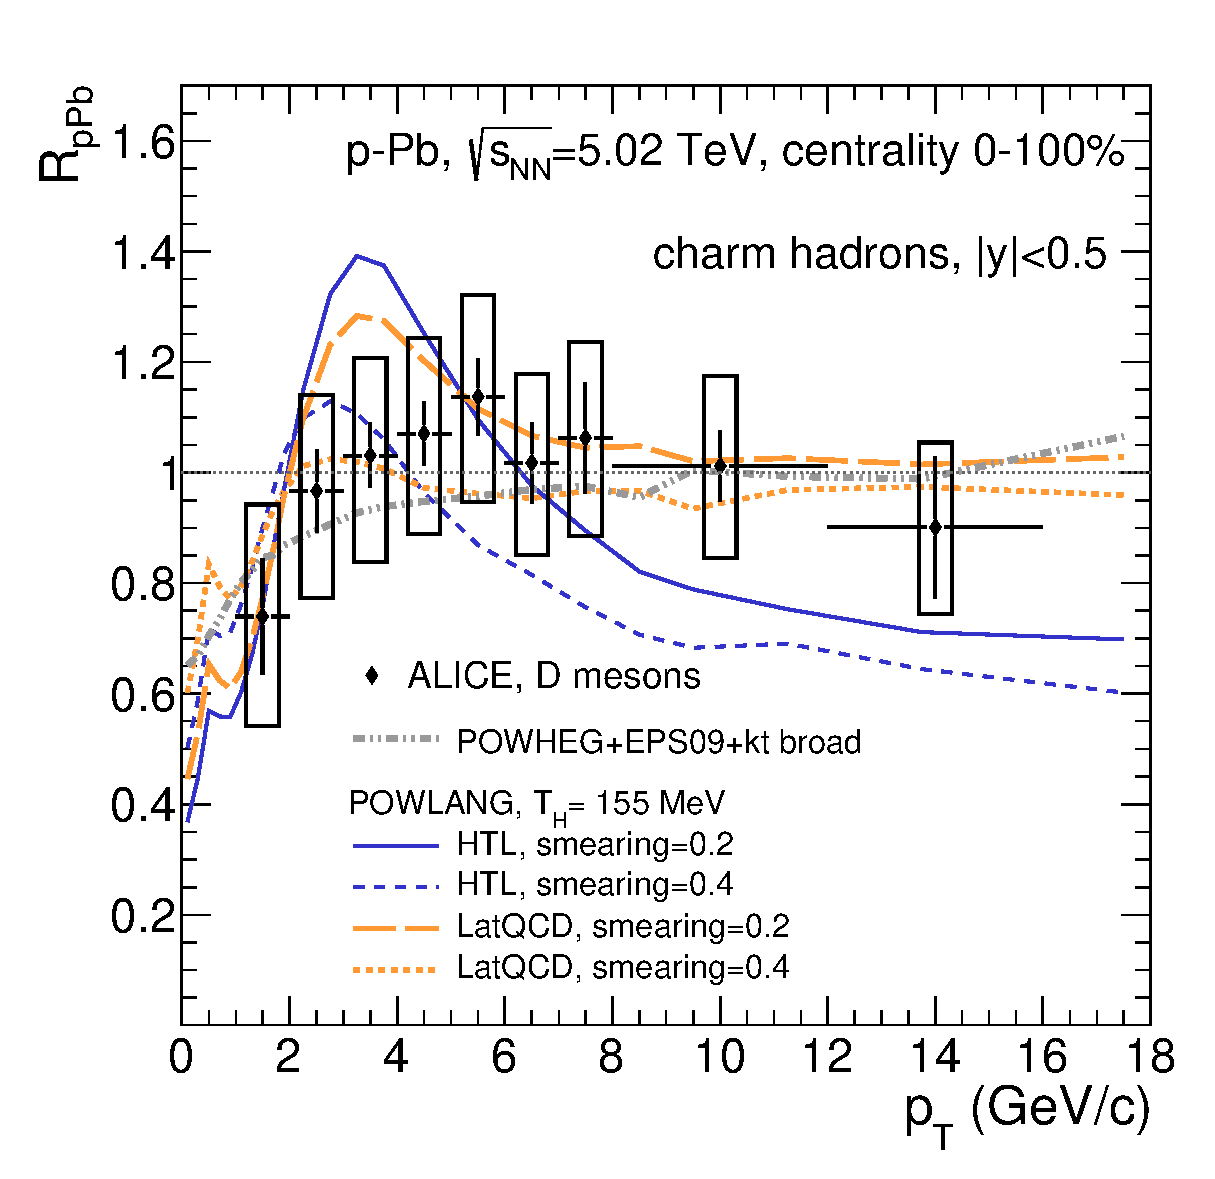
\includegraphics[width=0.4\textwidth]{hf/figures/RpA-Lang-HTLvsLatQCD-Data-EPS09.eps}
%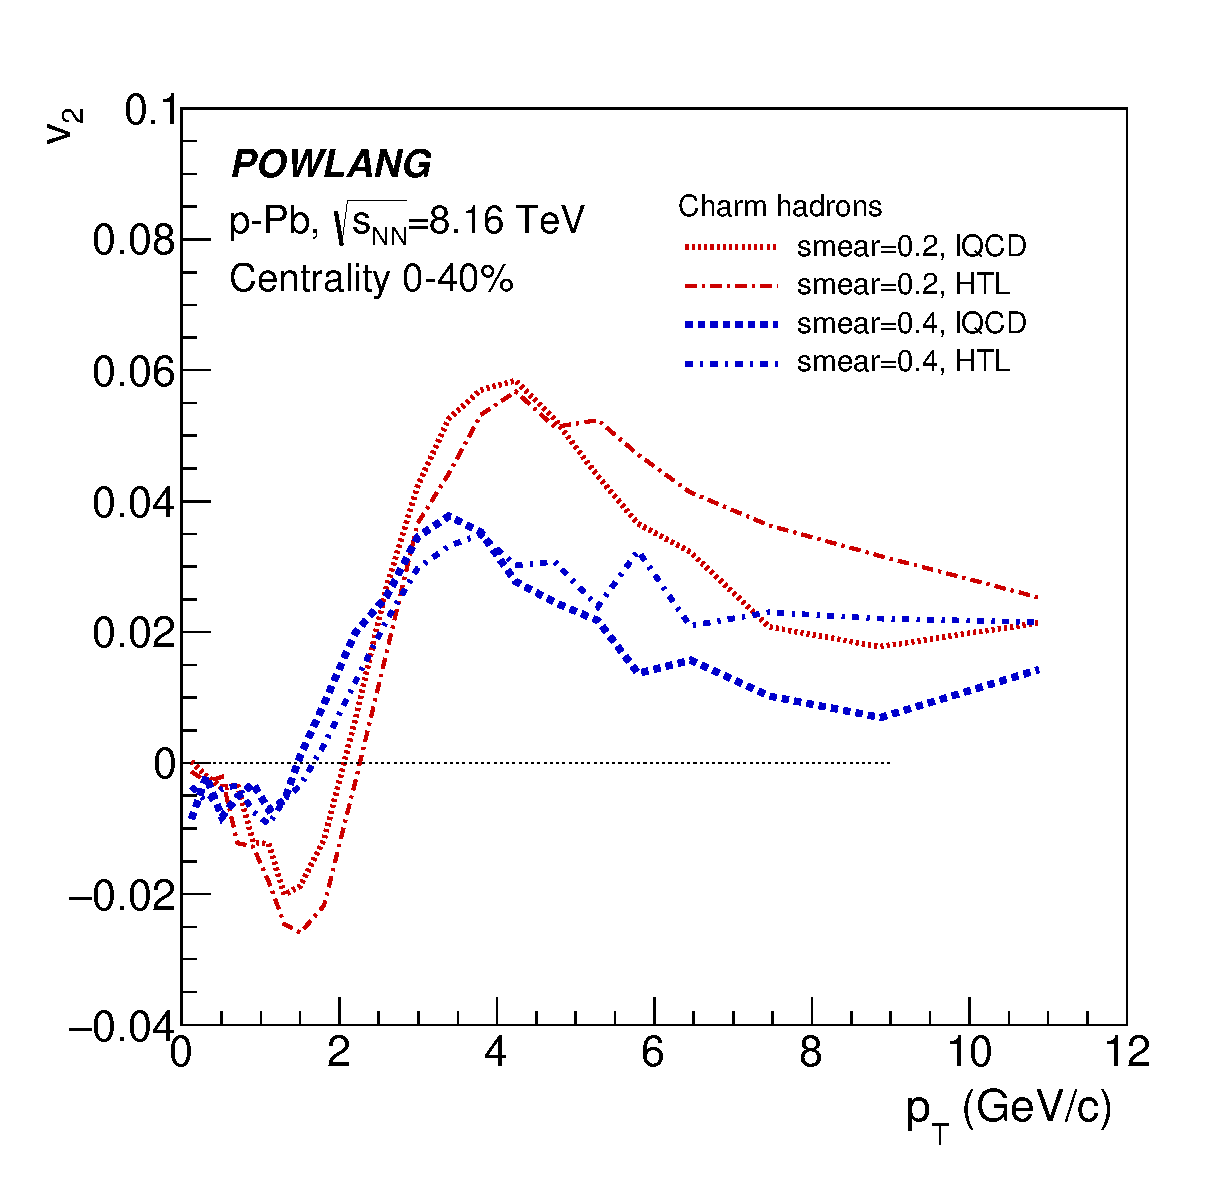
\includegraphics[width=0.3\textwidth]{hf/figures/v2cD_pPb8TeV_smear.eps}
%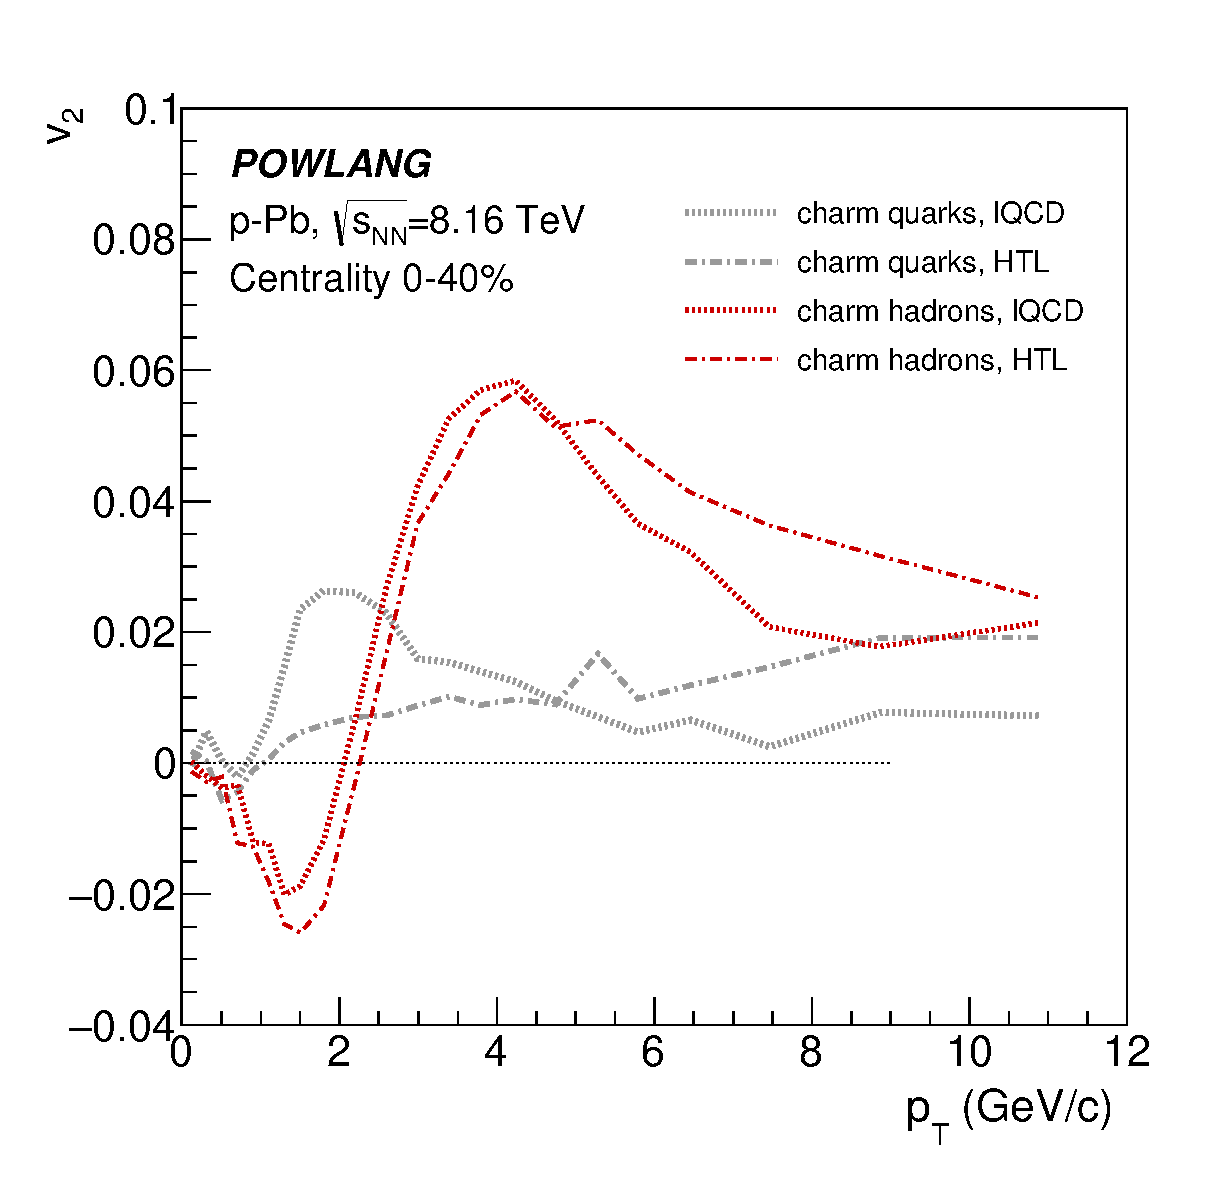
\includegraphics[width=0.3\textwidth]{hf/figures/v2cD_pPb8TeV_HTLvslQCD.eps}
\caption{
%Left: The nuclear modification factor of electrons from heavy-flavour decays in the 0-20\% most central d-Au collisions at $\sqrt{s_{\rm NN}}\!=\!200$ GeV. 
Left: Nuclear modification factor of B mesons in p--Pb collisions
Right: The nuclear modification factor of charmed hadrons in p--Pb collisions at $\sqrt{s_{\rm NN}}\!=\!5.02$ TeV. Results of the POWLANG model with different choices of the transport coefficients and of the smearing of the initial condition are shown and compared to ALICE results (to be updated for Beauty RpPB). Also reported, in grey, the curve containing only cold-nuclear-matter effect.
%Centre: The elliptic flow of charmed hadrons in the 0-40\% most central p-Pb collisions at $\sqrt{s_{\rm NN}}\!=\!8.16$ TeV. Results of the POWLANG model with different choices of the transport coefficients and of the smearing of the initial condition are shown. 
%Right: a comparison of the results at the level of charm quarks and hadrons. An important fraction of the flow is acquired at hadronization via recombination with light partons from the medium (could make a unique picture with POWLANG scenarios).
}
\label{fig:POWLANG-small1}
\end{figure}
%%%%%%%%%%%%%%%%%%%%%%%%%%%%%%%%%%%%%%%%%%%%%%%%%%%%%%%
\begin{figure}[ht]
\centering
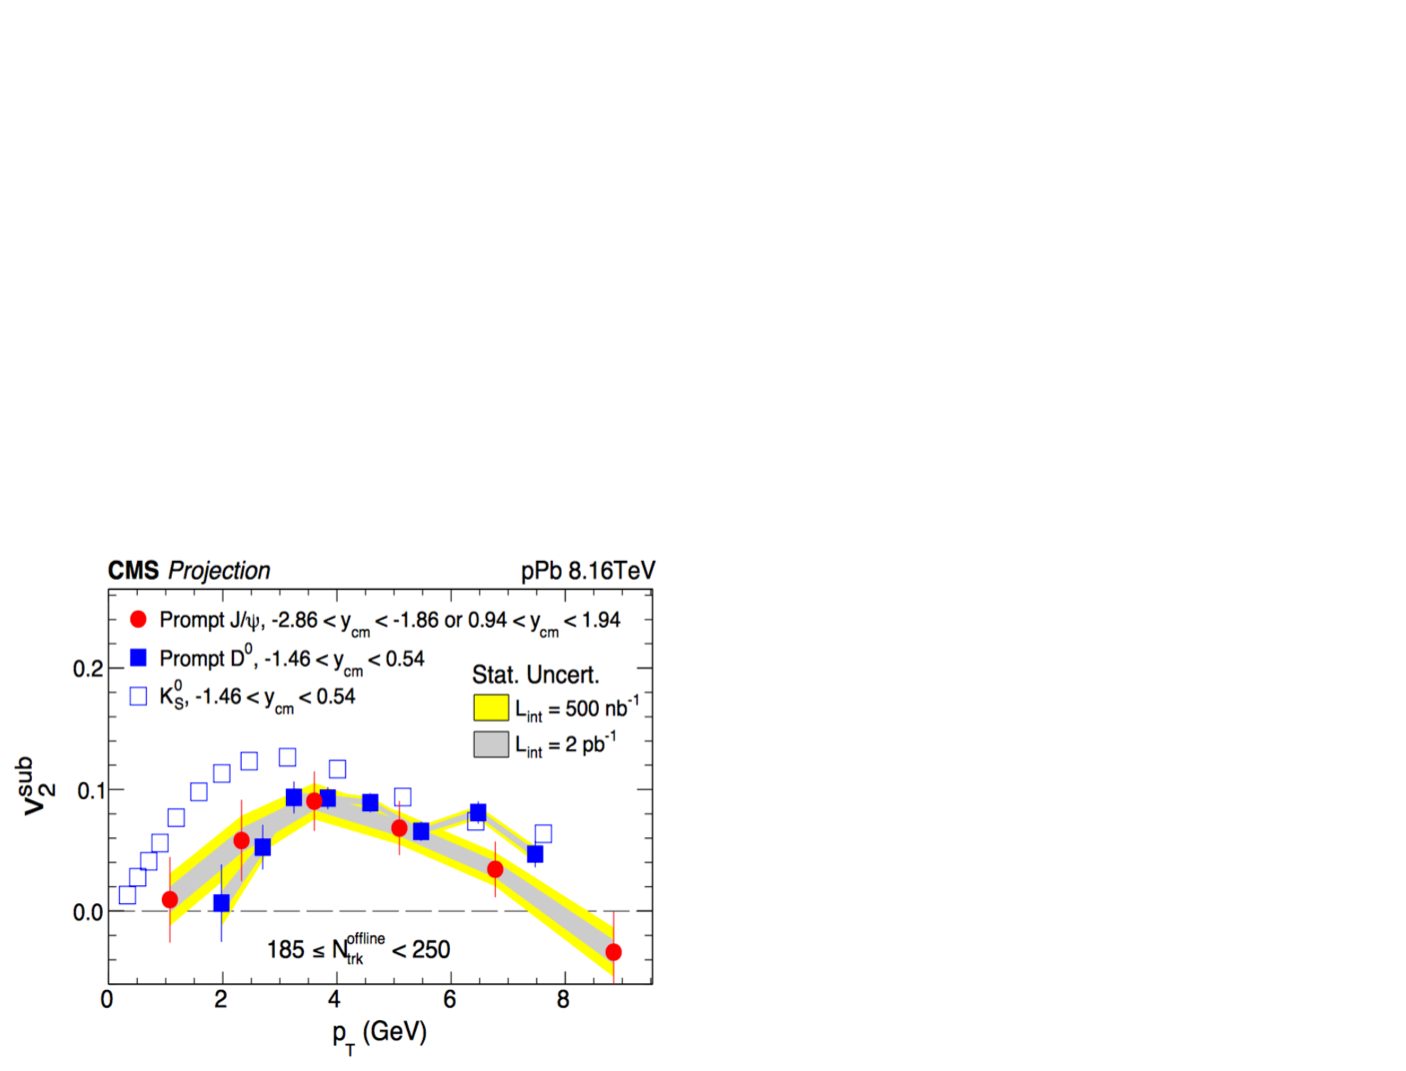
\includegraphics[width=0.4\textwidth]{hf/figures/CMS_Dv2.pdf}
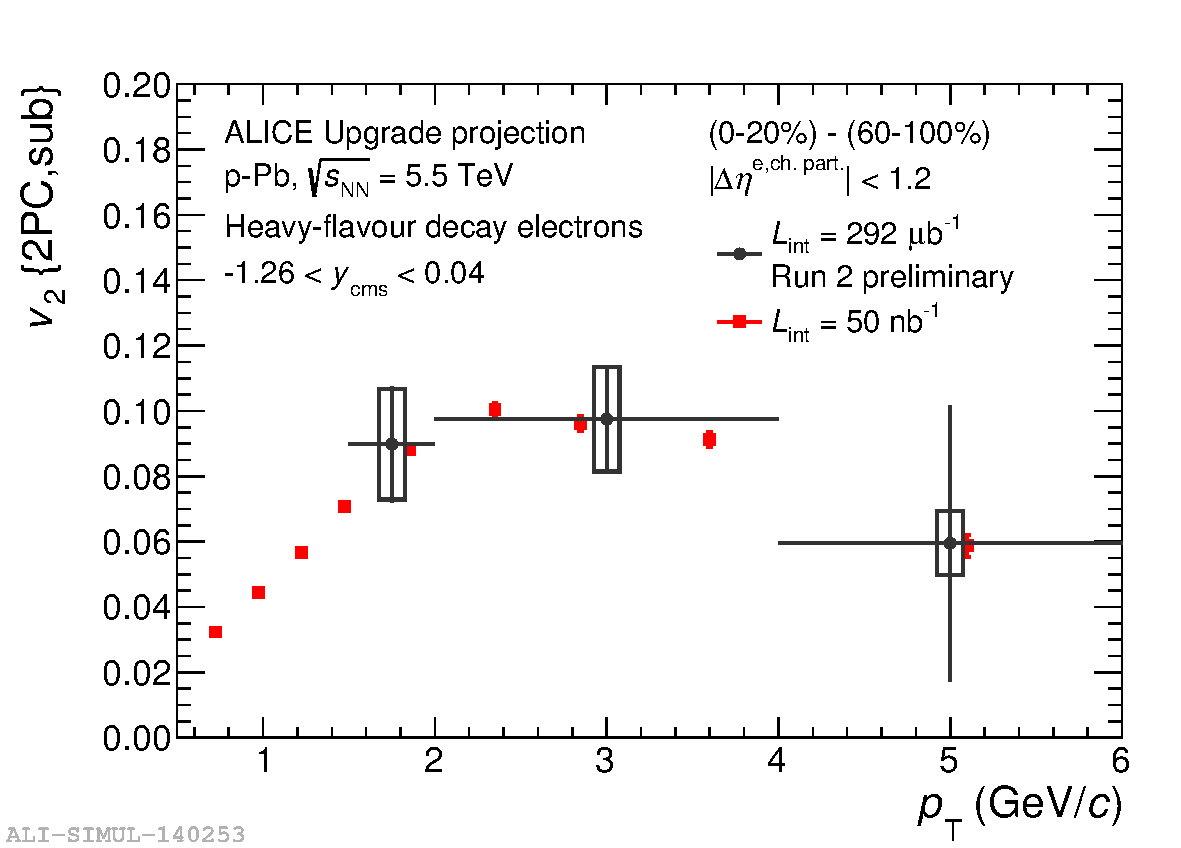
\includegraphics[width=0.4\textwidth]{hf/figures/2017-Oct-30-HFev2Plot.pdf}
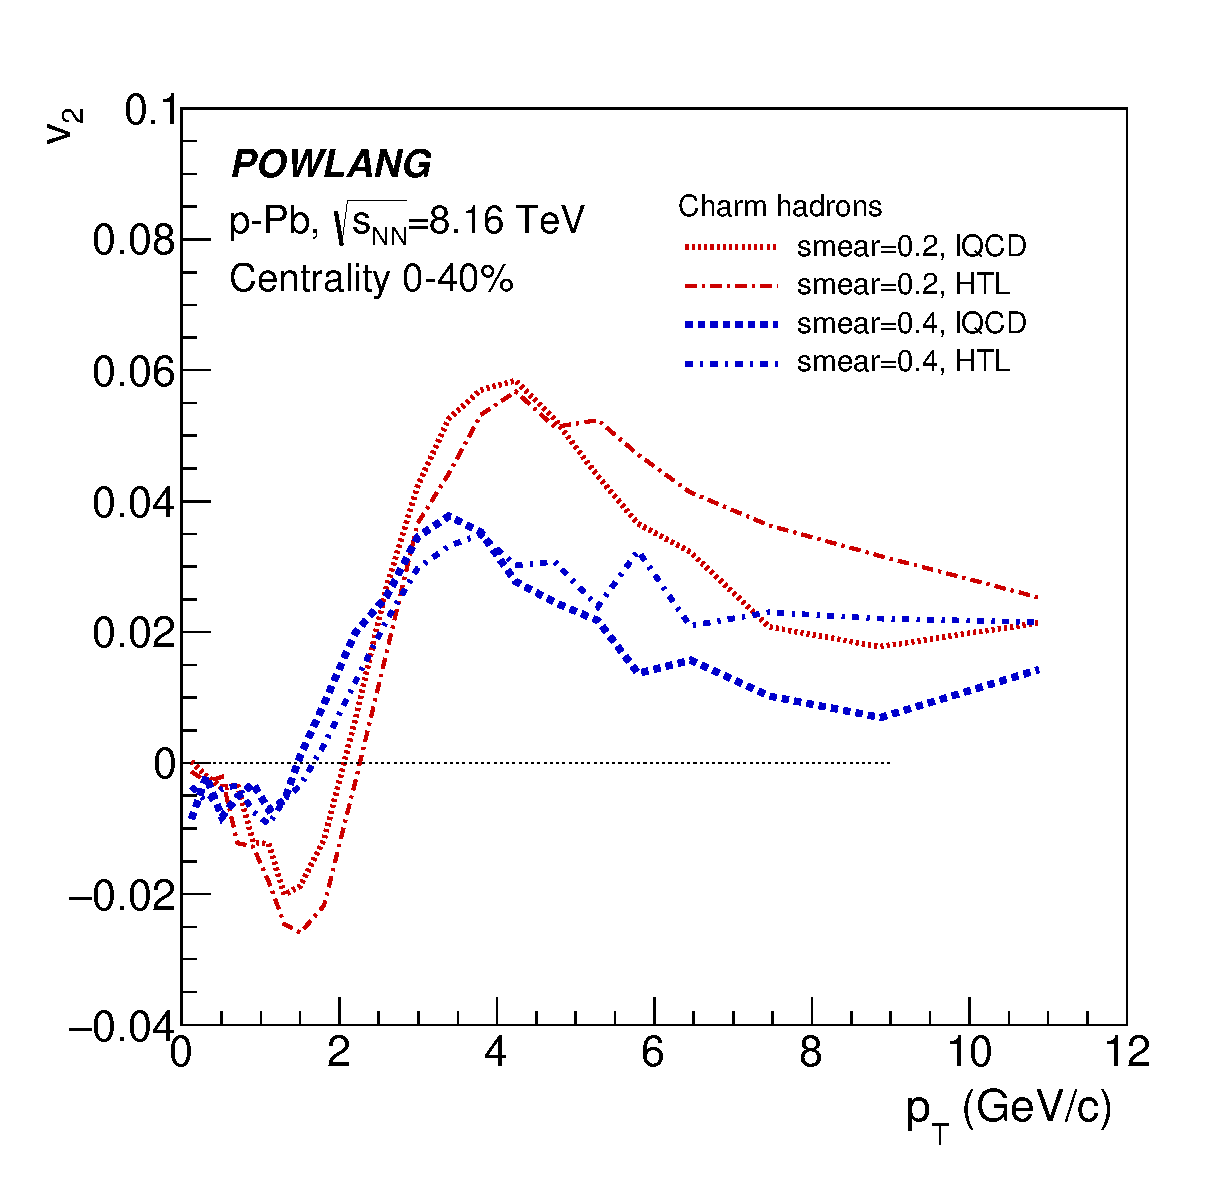
\includegraphics[width=0.4\textwidth]{hf/figures/v2cD_pPb8TeV_smear.eps}
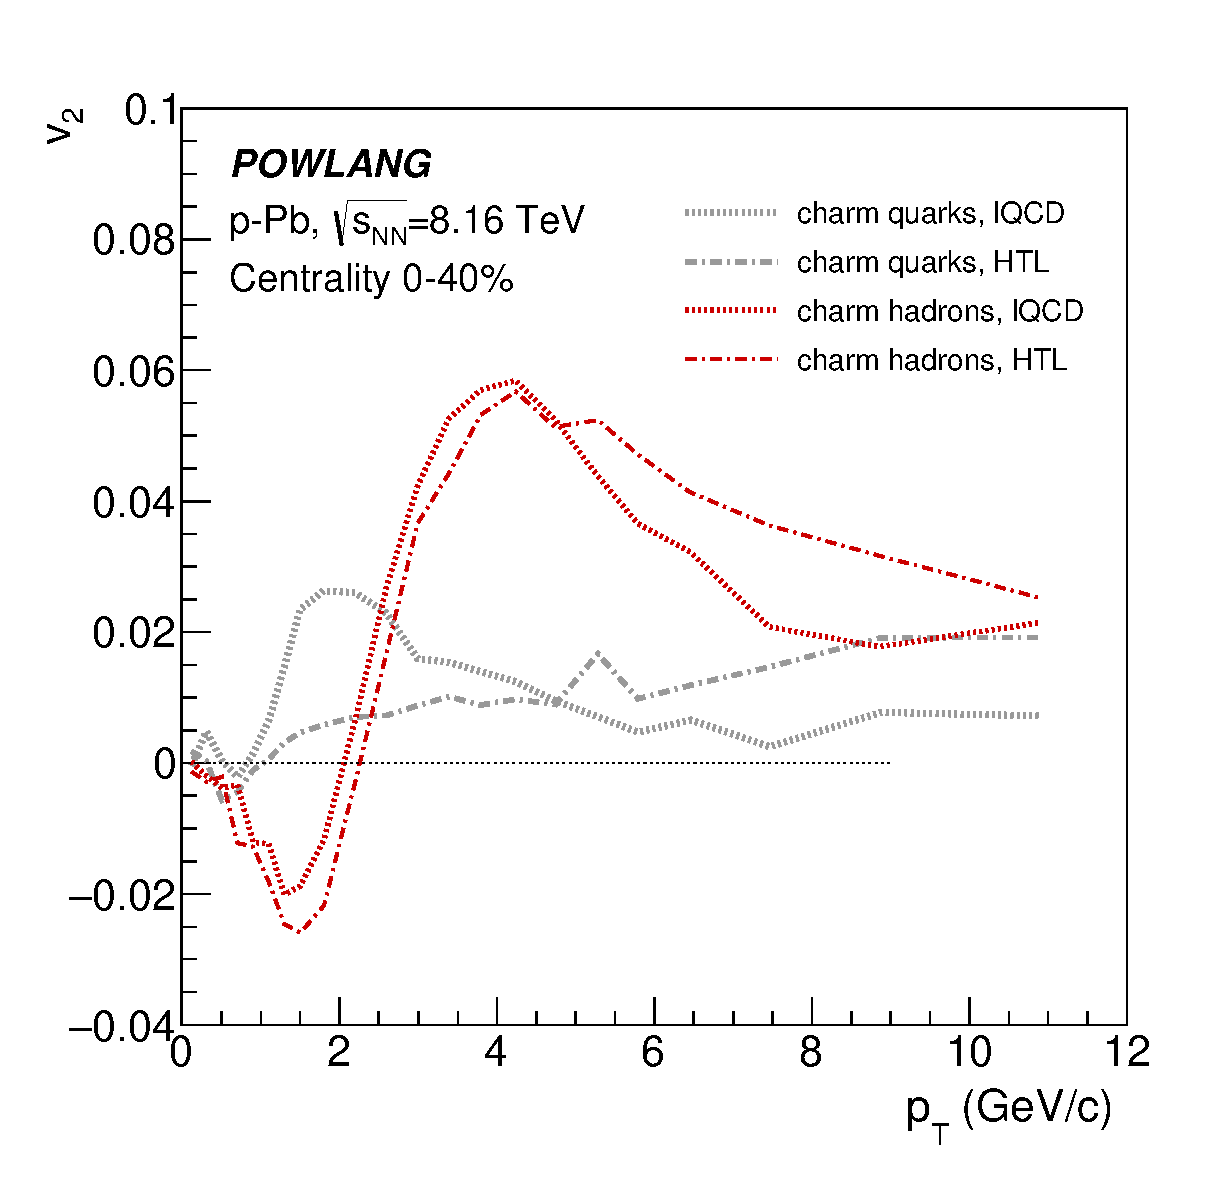
\includegraphics[width=0.4\textwidth]{hf/figures/v2cD_pPb8TeV_HTLvslQCD.eps}
\caption{
Left: The elliptic flow of charmed hadrons in the 0-40\% most central p-Pb collisions at $\sqrt{s_{\rm NN}}\!=\!8.16$ TeV. Results of the POWLANG model with different choices of the transport coefficients and of the smearing of the initial condition are shown. 
Right: a comparison of the results at the level of charm quarks and hadrons. An important fraction of the flow is acquired at hadronization via recombination with light partons from the medium.
Left: projection of D-meson elliptic flow as a function of $\pt$ in high-multiplicity p--Pb collisions at $\sqrtsNN=8.16$~$\UTeV$ with CMS.
Right: projection of elliptic flow of electrons from heavy-flavour hadron decays as a function of $\pt$ in 0--20\% central p--Pb collisions at $\sqrtsNN=5.02$~$\UTeV$ with ALICE.
\label{fig:POWLANG-small2}
\end{figure}
%%%%%%%%%%%%%%%%%%%%%%%%%%%%%%%%%%%%%%%%%%%%%%%%%%%%%%%%%%%
As an example of the findings which can be obtained within such a setup and of the systematic uncertainties by which they are affected, in Fig.~\ref{fig:POWLANG-small1} we display some results of the POWLANG model described in~\cite{Beraudo:2015wsd}.
In Fig.~\ref{fig:POWLANG-small1} results of transport calculations are compared to experimental data (projections) for the nuclear modification factor of D (B) mesons at the LHC. Notice how different choices of the transport coefficients (the ones provided by weak-coupling and lattice-QCD calculations were employed in~\cite{Beraudo:2015wsd}) and of the initial conditions (each nucleon-nucleon collision was assumed to deposit some energy with a Gaussian smearing in the transverse plane) affect the results. Notice also how, within their large systematic uncertainties, old experimental data for the nuclear modification factor would be also compatible with no final-state effect, as one can see from the grey curves which include only the effect of the nPDF's and of the initial $k_T$-broadening acquired in Cold-Nuclear-Matter. Hence, in order to distinguish among these (and possible others) various theoretical scenarios, an experimental effort in reducing the systematic errors has to be carried out.
As displayed in Fig.~\ref{fig:POWLANG-small2} the possible production of a hot deconfined medium in proton-nucleus collisions, modifying the propagation of the heavy quarks and their hadronization, would also leave its fingerprint in the azimuthal distribution of the final hadrons, leading in particular to a non-vanishing elliptic-flow coefficient. Notice how one gets a positive $v_2$ for charm hadrons only starting from $p_T\!\approx\!2$ GeV/c, in agreement with recent CMS data. The results depend quite strongly on the initial condition...For what concerns open-charm hadrons, the ones considered in [...]
The precision level achieved with the projections from CMS and ALICE with integrated luminosities $L_{int}=$ 2 $pb^{-1}$ for ATLAS and CMS and 1 $pb^{-1}$ with ALICE will will shed light on th different mechanisms behind the observed anisotropy (Fig.~\ref{fig:POWLANG-small2} for D mesons with CMS and electrons from heavy-flavour hadron decays with ALICE).


\begin{itemize}
\item{RpPb} (D, B, baryons): mid and fwd rapidity to constrain CNM/small QGP effects in wide kinematic range
\item{v2}  in high-multiplicity pPb (D, HF-decay electrons and muons) to constrain initial final state effects
\item{pp high-multiplicity} bridge between pp to PbPb to study HF production processes, onset of coalescence.
Theory connection crucial
\end{itemize}

\textbf{FIGURES}:
\begin{enumerate}
\item D RpA (ALICE,CMS, LHCb, ATLAS)
\item v2 in high mult pPb: CMS D0,  ALICE HF electrons, ATLAS D*
\item D-meson yields in high multiplicity pp (ALICE)
\item Theory predictions for v2 in high mult pp/pPb?
\end{enumerate}

